% \pdfoutput=1

\documentclass{webofc}
\usepackage[varg]{txfonts}   % Web of Conferences font

\usepackage{tikz}
\usetikzlibrary{arrows, calc, decorations.pathreplacing}

\usepackage[hidelinks]{hyperref}



%
% Put here some packages required or/and some personnal commands
%
%
\begin{document}
%
\title{Recent developments in histogram libraries}

\author{\firstname{Hans Peter} \lastname{Dembinski}\inst{1} \and
        \firstname{Jim} \lastname{Pivarski}\inst{2} \and
        \firstname{Henry} \lastname{Schreiner}\inst{2}\fnsep\thanks{\email{hschrein@cern.ch}}
        % etc.
}

\institute{
	Max Planck Institute for Nuclear Physics, Heidelberg, Germany
\and
    Princeton University, Princeton, USA
}

\abstract{%
Boost.Histogram, a header-only C++14 library that provides multi-dimensional histograms and profiles, became available in Boost 1.70. It is extensible, fast, and uses modern C++ features. Using template meta-programming, the most efficient code path for any given configuration is automatically selected. The library includes key features designed for the particle physics community, such as optional under- and overflow bins, weighted increments, reductions, growing axes, thread-safe filling, and memory-efficient counters with high-dynamic range.

Python bindings for Boost.Histogram are being developed in the Scikit-HEP project to provide a fast, easy-to-install package as a backend for other Python libraries and for advanced users to manipulate histograms. Versatile and efficient histogram filling, effective manipulation, multithreading support, and other features make this a powerful tool. This library has also driven package distribution efforts in Scikit-HEP, allowing binary packages hosted on PyPI to be available for a very wide variety of platforms.

Two other libraries fill out the remainder of the Scikit-HEP Python histogramming effort. Aghast is a library designed to provide conversions between different forms of histograms, enabling interaction between histogram libraries, often without an extra copy in memory. This enables a user to make a histogram in one library and then save it in another form, such as saving a Boost.Histogram in ROOT. And Hist is a library providing friendly, analyst-targeted syntax and shortcuts for quick manipulations and fast plotting using these two libraries.
}

\maketitle



\section{Introduction}
\label{intro}

There is no shortage of histogramming libraries for Python (see Table \ref{tab-libraries}). However, many/most of these are abandoned, have a narrow focus, and most importantly, have little or no interaction with other histogramming libraries. For the Scikit-HEP family of Python libraries~\cite{Eduardo:2019chep}, histogramming was identified as a weak point in the scientific Python stack that could be addressed directly in Scikit-HEP. At this time, a new histogramming library for C++ was being developed and was about to be proposed for inclusion in the Boost Libraries. Working together with the author of what would become Boost.Histogram via a thorough review and unanimous approval, a plan was devised to build a Python system for histogramming on top of Boost.Histogram. Together, these two closely related projects have been providing some of the most exciting developments in histogramming for HEP in recent years.

\begin{table}[h]
	\centering
	\caption{Histogram libraries for Python. For the PyPI column, ``Pure'' means the library is pure Python, ``Wheels'' means it is compiled but binary wheels are available, ``Source'' means the code is there, but must be compiled and may require other dependencies, and ``No'' means it is not hosted on PyPI. Old projects that predate universal (pure python) wheels may be incorrectly listed as ``Source''. Ordered by last update time, compiled near the end of 2019.}
	\label{tab-libraries}       % Give a unique label
	\small
	\begin{tabular}{llll}
		\hline
		Library                                                                      & Updated & PyPI   & Notes                                                \\ \hline
		\href{https://www.numpy.org/}{NumPy}                                         & 2019         & Wheels & Very simple histogramming functions                  \\
		\href{https://coffeateam.github.io/coffea/notebooks/histograms.html}{coffea} & 2019         & Pure   & Family of tools for HEP Columnar analysis            \\
		\href{https://histogrammar.org}{Histogrammar}                                & 2019         & Pure   & Multilanguage, limited support                       \\
		\href{https://pygram11.readthedocs.io}{pygram11}                             & 2019         & Wheels & Unix only, Python 3 only                             \\
		\href{https://root.cern.ch/pyroot}{PyROOT}                                   & 2019         & No     & CERN's ROOT, UNIX binaries on conda-forge            \\
		\href{https://yoda.hepforge.org}{YODA}                                       & 2019         & No     & HEP tool for MCnet                                   \\
		\href{https://physt.readthedocs.io/en/latest/tutorial.html}{physt}           & 2019         & Pure   & Non-HEP specific tool                                \\
		\href{https://github.com/astrofrog/fast-histogram}{fast-histogram}           & 2019         & Yes    & Fast but limited                                     \\
		\href{https://vaex.io}{Vaex}                                                 & 2019         & Source & Large system for data analysis                       \\
		\href{https://pypi.org/project/hdrhistogram/}{hdrhistogram}                  & 2019         & Source & Multilanguage, large range                           \\
		\href{https://pypi.org/project/multihist/}{multihist}                        & 2019         & Pure   & NumPy wrapper for syntax                             \\
		\href{https://github.com/scikit-hep/histbook}{HistBook}                      & 2018         & Pure   & Archived, Replaced by boost-histogram / hist         \\
		\href{https://pypi.org/project/qhist/}{qhist}                                & 2018         & Source & ROOT required, Python 2.7 only                       \\
		\href{https://github.com/theodoregoetz/histogram}{theodoregoetz}             & 2018         & No     & Tried to combine many of the below packages          \\
		\href{https://github.com/drdavis/rootplotlib}{rootplotlib}                   & 2016         & No     & ROOT backend                                         \\
		\href{https://pypi.org/project/matplotlib-hep/}{matplotlib-hep}              & 2016         & Source & Focused on plotting                                  \\
		\href{https://github.com/jpivarski/svgfig}{SVGFig}                           & 2016         & No     & Plotting framework                                   \\
		\href{https://github.com/jpivarski/plothon}{Plothon}                         & 2015         & No     & Predecessor to SVGFig                                \\
		\href{https://pypi.org/project/pyhistogram/}{pyhistogram}                    & 2014         & Pure   & Inspired by rootpy                                   \\
		\href{https://pypi.org/project/pypeaks}{pypeaks}                             & 2014         & Pure   & Peak detection                                       \\
		\href{https://github.com/opendatagroup/cassius}{Cassius}                     & 2013         & No     & Statistical Modeling Package                         \\
		\href{https://pypi.org/project/histogramy}{histogramy}                       & 2013         & Pure   & 1D with some fitting tools                           \\
		\href{https://pypi.org/project/histogram}{histogram}                         & 2011         & Source & For Distributed Data Analysis for Neutron Scattering \\
		\href{https://pypi.org/project/SimpleHist/}{SimpleHist}                      & 2011         & Pure   & NumPy based                                          \\
		\href{https://pypi.org/project/paida/}{paida}                                & 2007         & Source & Analysis and plotting                                \\ \hline
	\end{tabular}
\end{table}


\section{Boost.Histogram for C++}
\label{sec-bh-cpp}

% Ideas:
%
% * Basic overview
% * Include everything mentioned in abstract if possible: optional under- and overflow bins, weighted increments, reductions, growing axes, thread-safe filling, and memory-efficient counters with high-dynamic range.
% * Highlight dynamic features that enable Python (or other) bindings (handy place to highlight compile time benefits when dynamic axes, etc not needed)
% * Describe 1.72's high performance .fill
% * Include performance plot from slides, diagram from slides (I can add images to repo later - Henry)

Boost.Histogram is a header-only C++14 library which implements feature-rich multi-dimensional generalized histograms. It is part of the \href{https://www.boost.org/}{Boost C++ Libraries} and only depends on a few other header-only libraries from the Boost project and the C++ standard library. The feature set of Boost.Histogram was designed with the needs of the (astro)particle physics community and the wider data analysis community in mind. In particular, feature parity with the histogram implementations from the \href{https://root.cern.ch/}{ROOT framework}~\cite{Brun:1997pa} and the \href{https://www.gnu.org/software/gsl/}{GNU Scientific Library}~\cite{gough2009gnu} was a central goal.

The library was designed to be easy to use for the casual user, while offering a high amount of flexibility and extensibility for the power user. In a classic C++ design based on run-time polymorphism, flexibility and extensibility comes at the cost of performance. Boost.Histogram avoids the run-time trade-off and achieves higher performance than other libraries with static polymorphism based on templates and modern template meta-programming.

Compatibility with other Boost libraries and the C++ standard library was another central design goal. By adhering to standard interfaces, the library avoids duplicating functionality provided by other libraries, especially the standard library. For example, these are one-liners:
\begin{itemize}
\item Sum all counts with \verb|std::accumulate|.
\item Find the cell with the highest count with \verb|std::max_element|.
\item Compute the cumulative distribution with \verb|std::partial_sum|.
\end{itemize}

\begin{figure}[h]
	\begin{center}
        \begin{tikzpicture}[every path/.style={thick}, scale=.7]
		
		% Main grid
		\draw (-2,-2) rectangle (2,2);
		\foreach \i in {-1,0,1} {
			\draw (-2,\i) -- (2,\i);
		}
		\foreach \i in {-1.50465122, -0.76393202,  0.34370152} {
			\draw (\i, -2) -- (\i, 2);
		}
		\draw [latex-] (2,2) -- (2.4,2.2) node [right] {Storage $\begin{pmatrix}\textrm{Static}\\ \textrm{Dynamic}\end{pmatrix}$};
		
		% Left axis
		\draw (-2.3,-2) -- (-2.3,2);
		\foreach \i in {-2,-1,0,1,2} {
			\draw (-2.45,\i) -- (-2.15,\i);
		}
		\node at (-2.3,2) [above] {Regular axis};
		
		% Bottom axis
		\draw (-2,-2.3) -- (2,-2.3);
		\foreach \i in {-2.        , -1.50465122, -0.76393202,  0.34370152,  2.} {
			\draw (\i, -2.45) -- (\i, -2.15);
		}
		\node at (2,-2.2) [right=.4cm, align=left] {Regular axis with\\log transform};
		
		% Axes
		\begin{scope}[xshift=-2.9cm, yshift=-2.3cm, rotate=45]
		\draw [decorate, decoration={brace,amplitude=10pt}, xshift=-4pt, yshift=0pt]
		(0.5,-0.7) -- (0.5,0.7);
		\node at (-.3,0) {axes};
		\end{scope}
		
		% Overflow bin
		\draw (2.05,-2.3) -- (2.4, -2.3);
		\draw (2.4, -2.45) -- (2.4, -2.15);
		\draw [latex- ] (2.2, -2.3) -- (2.2, -2.6) node [below] {Optional overflow};
		
		% Underflow bin
		\draw (-2.05,-2.3) -- (-2.4, -2.3);
		\draw (-2.4, -2.45) -- (-2.4, -2.15);
		\draw [latex-] (-2.25, -2.3) -- (-1.8, -2.6) node [below] {Optional underflow};
		
		% Accumulators
		\node (accum) at (1.2,1.5) [circle, minimum width=.7cm, draw] {};
		\draw [latex-] (accum) -- (2.25, .5) node [right, align=left] {Accumulator\\int, double,\\unlimited, ...};
		
		\end{tikzpicture}
		\caption{Components of a histogram. Zero or more axes (two shown) are combined with a storage. Each item stores an accumulator.}
		\label{fig-design}
	\end{center}
	
\end{figure}

\subsection{Generalized histograms}
\label{sec-bh-cpp-gen}

A histogram in the common sense (see Figure \ref{fig-design}) is a collection of counts $n_i$, where each is associated to an interval out of a sequence of non-overlapping consecutive intervals, called \emph{bins}. When a value $x$ is passed to a histogram, the bin $i$ is found which contains $x$ and the associated count $n_i$ is incremented. A multi-dimensional histogram accepts value tuples $(x, y, z, \dots)$. For each value in the tuple an independent sequence of bins exists, which we call an \emph{axis}. The count is now looked up based on a multi-dimensional index $(i,j,k,\dots)$ obtained from the mappings $(x \rightarrow i, y \rightarrow j, z \rightarrow k, \dots)$.

Boost.Histogram generalizes the classic histogram concept in three ways.

\begin{description}

    \item[Custom axis objects.] The mapping from input value to index provided by an axis $x \rightarrow i$ can be completely user-defined. Values are not restricted to numbers; arbitrary C++ objects can be used as values when an appropriate mapping is provided, for example, strings can be used. Bins do not have to be consecutive, they can have gaps and arbitrary hyperdimensional shapes. Hexagonal binning is possible, or bins that are HEALPix\footnote{\underline{H}ierarchical \underline{E}qual \underline{A}rea iso\underline{L}atitude \underline{Pix}elation of a sphere.} pixels~\cite{gorski2005healpix} (although neither are currently implemented in the core library).

\item[Custom accumulators.] The counts in a generalized histogram can be replaced by user-defined accumulators. Accumulators can take any number of \emph{samples} which, like values, can be arbitrary C++ objects. Values and samples are passed to the generalized histogram together; values are converted to indices which address the accumulator, and samples are passed to the accumulator. The library provides a few standard accumulators, such as accumulators to compute mean and variance of samples in each bin. This is called a \emph{profile} in the ROOT framework and is a separate class, while it is just a choice of accumulator in a normal histogram in Boost.Histogram.

\item[Custom storages.] It is possible to completely customize how counts (or accumulators) are allocated and addressed in memory. The sub-component responsible for this is called a \emph{storage}. The histogram class converts the multi-dimensional index $(i,j,k,\dots)$ into a single linear index, which is passed to the storage. The standard storage allocates memory upfront for all cells and places the counts sequentially in memory, using the linear index as a memory offset. This gives the best look-up performance and is space-efficient for densely filled histograms, since it is not necessary to store the linear index explicitly for each cell. The downside of dense storage is that all cells take up space, even if they contain zero counts. The library also supports sparse storage based on an STL-compliant hash map. Only cells with non-zero counts use space in such a sparse storage, but each cell has to store its linear index in addition to the payload and incurs some overhead for hash-based addressing.

The memory allocation strategy of a storage can be customized as well. The standard storage allocates memory dynamically from the heap, but the library has builtin support for a storage based on a fixed-size stack-based memory buffer. The latter allows one to efficiently create and destroy many small histograms, for example. The builtin \verb|unlimited_storage| dynamically allocates memory to grow the counter capacity as needed, starting with a single byte per cell up to arbitrarily many bytes (limited by available memory only). This storage offers a unique no-overflow-guarantee and is memory-efficient in high dimensions, where the number of cells is large and the small memory footprint per cell pays off.
\end{description}

The three sub-components of a generalized histogram, axis types, storages, and accumulators, are orthogonal. This means that any sub-component can be replaced or modified independently of the others. Orthogonal design is very powerful since it offers a huge customization potential from all possible combinations.

\subsection{Notable features}
\label{sec-bh-cpp-feat}

We briefly list some of the other notable features here.

\begin{description}
\item[Arithmetic operators.] Histograms support the standard math operators \verb|+|, \verb|-|, \verb|*|, and \verb|/|.

\item[Growing axes.] A standard axis has a fixed value range and number of bins, defined at the time of construction. The library also supports growing axes; such an axis has an initial range and bin number but grows with the input. If a value is encountered that would fall outside of the axis range, the axis range is extended to contain the value and the number of bins is increased.

\item[Optional underflow and overflow bins.] Each axis of the histogram can have optional underflow and overflow bins. These are extra bins beyond the defined range of the axis that count all values which fall below the smallest value on the axis or above the largest value, respectively. The existence or absence of these bins is mostly transparent for the user. They are very useful to detect outliers and to offer lossless reductions (explained below).

\item[Reductions.] The library offers tools to reduce the memory footprint of a histogram by reducing the number of bins of an axis or by completely removing an axis. The number of bins in an axis can be reduced by shrinking its value range and/or by merging any number of adjacent bins into one larger bin. Likewise, an axis can be removed completely by summing over its bins (a so called \emph{projection}). In both cases, the presence of underflow and overflow bins guarantees that the reduced histogram is identical to one obtained by filling with the original values. This is not generally possible when underflow and overflow bins are missing.

\item[Thread-safe filling of histograms.] Filling histograms with values is not thread-safe in general, but the library offers a builtin thread-safe counter based on a \verb|std::atomic| integer type and a thread-safe locking infrastructure for storages; the latter is needed when growing axes are present, which can trigger a resizing of the storage.

\item[Static and dynamic axis configuration.] The library supports both histograms with static and dynamic axis containers. A histogram with a static axis container is fixed at compile-time in the number and types of axes. The number and axis types can vary at run-time for a dynamic axis holder. The static axis container produces histograms which are more performant, as the compiler can find more opportunities to optimize the code. When Boost.Histogram is used as a backend in a run-time environment like Python, however, axes must be configurable at run-time. The performance difference vanishes when the histogram is filled with chunks of values at once, see next item.

\item[Filling individual values and chunks of values.] Histograms can be filled with one value at once or by passing a contiguous chunk of values at once. Both cases are handled by separate code segments, which were highly optimized for performance. Passing contiguous chunks of values is up to five times faster for chunks of moderate size (32768 values) than filling one value at a time, and therefore preferred when chunks are available. Using the chunk code for single values would be slow, however, and therefore the other optimized code path exists.
\end{description}

\section{boost-histogram for Python}
\label{sec-bhp-intro}

Boost.Histogram was developed with Python in mind. Original prototype bindings using Boost.Python were included in the draft first submitted to Boost; however, to keep the library focused they were removed before the library was accepted. New bindings based on PyBind11 were developed as part of the Scikit-HEP family of Python packages.

The new bindings were designed around four key ideas based on a study of the libraries in Table~\ref{tab-libraries}: \emph{Design}, \emph{Flexibility}, \emph{Speed}, and \emph{Distribution}. No single existing library provided a strong entry in all four of these areas.

\subsection{Design}
\label{sec-bhp-design}

The design of boost-histogram follows Boost.Histogram closely, with appropriate changes to adapt to Python and interactive usage. The description of a Histogram matches that described in Section~\ref{sec-bh-cpp-gen}.

The features listed in Section~\ref{sec-bh-cpp-feat} are mostly available to Python users. Python histograms support \textbf{arithmetic operators}. Most axis types support \textbf{growing axes} and \textbf{optional underflow and overflow bins}. The special storage that enables \textbf{thread-safe filling of histograms} is provided. And, since Python is a dynamic language, the bindings take advantage of \textbf{dynamic axis configuration} to set up all histograms. The other features adapted or specific to Python are listed below.

\begin{description}
\item[Filling with chunks of values.] The Python library supports filling contiguous chunks of values, based on the Boost.Histogram C++ feature. Since this looks like a NumPy array operation~\cite{walt2011numpy}, the differences should be noted. The data to be filled must be in the correct format (doubles or ints), and must be continuous (slices and other operations in NumPy can create arrays with strides, and Boost.Histogram's fill feature does not operate on strides). If these conditions are not met, a copy is made, affecting the performance and memory usage slightly.
\item[UHI (reductions).] Unified Histogram Indexing (UHI) was developed to provide a way for histograms to be manipulated and reduced in Python in a natural, concise way, and to decouple the ``tags'' describing actions and the histogram library performing the actions. Custom actions can be developed by users. See Section~\ref{sec-bhp-uhi} for more details.
\item[Python interaction.] Histograms (and the other objects provided) support the standard Python copy, deepcopy, and pickle protocols, and have docstrings, signatures (enhanced in Python 3), IPython keyboard completions, and natural textual representation,  providing a native experience for Python.
\item[NumPy interaction.] Special care went into making the library interact gracefully with NumPy. The underlying bin data for even accumulator based storages is available via mutable, no copy access. The Histogram object conforms to the Python buffer protocol. A special method is provided to produce NumPy style output tuples. For input, boost-histogram provides a NumPy module that provides functions identical to the three NumPy histogram functions, but powered by boost-histogram (and as such, up to 10 times faster than native NumPy histograms), and with extra keyword only arguments to provide a way to return boost-histogram objects instead of tuples.

\end{description}


\subsubsection{UHI}
\label{sec-bhp-uhi}

\textbf{Unified Histogram Indexing} (UHI) was inspired by an early design for Aghast (see Section~\ref{sec-aghast}). The key advancement in UHI was the design of a general API for providing ``tag'' types that can be used to perform operations in indexing. These tags can be provided by one library and used by another, and new tags can be written by users. And indexing is carefully designed to either behave like a NumPy array index if the syntax is allowed on both arrays and histograms, or to give an error on one or the other. The goal was to minimize situations where indexing will silently fail if you interchange histograms and arrays.

UHI allows single bin and array setting and accessing, and even provides optional access to the flow bins when setting. The third element of the Python slice syntax is used to perform actions on axes, such as rebinning or summation. While not currently implemented in version 0.6.2, the UHI specification includes arbitrary actions on axes. UHI was originally designed to provide an action per axis, though later based on user requests, it was expanded to allow a mapping to be provided, allowing a small number of axes to be operated on without having to explicitly list every axis.

\subsubsection{Axes}
\label{sec-bhp-axes}

Axes are available in a special augmented tuple. This tuple can accept any method a single axis can, and performs the property access or the method call on each axis, returning a tuple or ndarray as appropriate. This reduces many traditionally complex procedures into a simple, concise one or two lines.

\subsection{Flexibility}

Great care was taken to keep the incredible flexibility of Boost.Histogram intact in a dynamic, pre-compiled environment. A collection of over 20 axis types is provided, including \textbf{Regular} binning, \textbf{Integer} binning, and \textbf{Variable} binning, each with variants for underflow/overflow and growth. Both integer and string category axes are provided, also with optional growth. And regular binning can have a \textbf{transform} applied; the transform can be created by the user with a compiled callback using a language like Numba~\cite{lam2015numba} with a maximum of about 7\% penalty in speed over a precompiled function in C++.

Seven storages are provided as well, including three ``complex'' storages made from accumulators. The \textbf{Weight} storage provides high precision weighted sums that track the count as well. The \textbf{Mean} and \textbf{WeightedMean} storages can be used to produce ``profile'' histograms that track the average of a weight in each bin, rather than the total number of entries observed. In some situations, a N-dimensional profile can replace a N+1-dimensional histogram.

\subsection{Speed}

Performance of the library was a key design consideration. For a significantly large 1D dataset, boost-histogram was measured to be 2.4 times faster than NumPy for regular bin spacing, which NumPy is also optimized for in 1D. For a 2D dataset, NumPy does not have special optimizations for regular binning, and in that case boost-histogram is 13 times faster. Both tests were performed with a single thread; with multithreaded filling boost-histogram was observed to gain another factor of 2-4, depending on the number of physical threads available on the hardware and the scale of the problem.

\subsection{Distribution}

To be used in the modern scientific Python ecosystem, a library must fulfill a variety of packaging criteria. All modern packages should be hosted on PyPI.org and should provide \textbf{wheels}. Pure Python packages only need to provide a ``universal wheel'', but compiled packages like boost-histogram need to provide a collection of wheels, one for each Python version and each supported platform. A system was developed for boost-histogram to build these wheels on the Azure DevOps cloud platform Continuous Integration (CI) system; these are automatically built whenever a new release is made via a manual request in the web API. The system developed for boost-histogram is now directly in use by at least three other Scikit-HEP packages.

One of the challenges unique to boost-histogram was the need for C++14 support by the compiler; the classic ``ManyLinux1'' wheels were not sufficient for compiling boost-histogram. The new ManyLinux2010 format was being finalized while this was being developed, but the older ManyLinux1 specification was still in heavy use 
(primary due to older versions of pip, the package installer for Python), so a special docker image was created that has a newer compiler but mostly conforms to ManyLinux1. This allows boost-histogram to support both specifications.

The wheel building system (and therefore boost-histogram) supports Python 2.7 and Python 3.6 through 3.8 on 64-bit architectures. On Linux systems, it also supports Python 3.5, partially because the infrastructure is already there in the official tooling and Linux tends to have older Python versions available in official channels. For ManyLinux1 and Windows, 32-bit architectures are also supported. As an organization, Scikit-HEP has agreed on a slightly modified version of NumPy Enhancement Proposal (NEP) 29, which outlines a community Python version support policy. Future versions of boost-histogram retain the right to remove versions that are no longer supported under that plan; the wheel building tools provide the ability to select versions and platforms for each project.

If a user is on an unsupported platform, such as specialized Linux distributions like ClearLinux or Alpine, the only requirements to build boost-histogram are a C++14 compatible compiler. Every dependency is header-only and supplied in the source tarball available on PyPI or via git submodules when building from the source repository.

Another way to distribute packages that has strong community adoption in the sciences and is rapidly gaining support in HEP is Conda. Conda is an alternative package manager designed to supply binary packages to a wide variety of systems. In contrast to pip, Conda never builds from source on the target machine, is less Python-centric, and provides a complete compiler stack with minimal dependencies on the underlying system. The most popular community source of packages and build infrastructure, Conda-forge has successfully been used to provide a complete ROOT build in for HEP~\cite{Burr:2019chep}, and is being used to supply a growing number of HEP packages, both with and without Python. Conda-forge packages of boost-histogram cover all supported targets of Conda-forge except for the rapidly disappearing Python 2.7 on Windows target; supported platforms include ARM and PowerPC.

\section{The Scikit-HEP family}
\label{sec-3}

The boost-histogram project is part of a larger plan for the Scikit-HEP family of tools (see Figure~\ref{fig-scikit-plan}).

\begin{figure}[h]
\begin{center}
	\vspace{-.75em}
	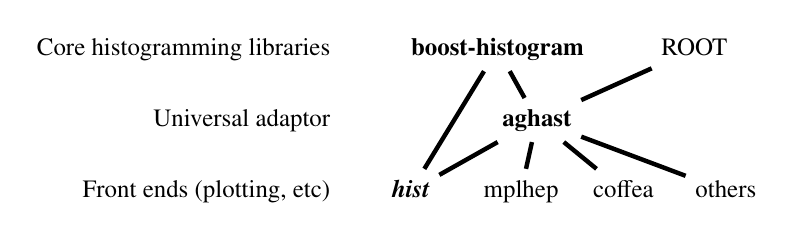
\begin{tikzpicture}[every path/.style={font=\vphantom{yH}\small}, yscale=.9]
	
	\begin{scope}
	\node at (-2.5,0) [left] {Core histogramming libraries};
	\node (bh) at (-.5,0)    {\bf boost-histogram};
	\node (root) at (2,0) {ROOT};
	\end{scope}
	
	\begin{scope}[yshift=-1cm]
	\node at (-2.5,0) [left] {Universal adaptor};
	\node (aghast) at (0,0)  {\bf aghast};
	\end{scope}
	
	\begin{scope}[yshift=-2cm]
	\node at (-2.5,0)     [left] {Front ends (plotting, etc)};
	\node (hist) at (-1.6,0)     {\textbf{\textit{hist}}};
	\node (mplhep) at (-.2,0)    {mplhep};
	\node (physt) at (1.1,0)     {coffea};
	\node (others) at (2.4,0)    {others};
	\end{scope}
	
	\begin{scope}[ultra thick]
	\draw (bh) -- (aghast);
	\draw (root) -- (aghast);
	\draw (mplhep) -- (aghast);
	\draw (hist) -- (aghast);i
	\draw (hist) -- (bh);
	\draw (physt) -- (aghast);
	\draw (others) -- (aghast);
	\end{scope}
	\end{tikzpicture}
	\vspace{-1.75em}
\end{center}
\caption{Plan for Scikit-HEP projects and relationship between them.}
\label{fig-scikit-plan}
\end{figure}


\subsection{Aghast}
\label{sec-aghast}

Aghast is a histogramming library that does not fill histograms and does not plot them. It is a conversion library, designed to make all the other histogramming libraries talk together. It defines an in-memory format for histograms, using flatbuffers. It understands a superset of all the functionality and binning methods that the other libraries support, and therefore can convert between them. It can convert to and from boost-histogram, ROOT (without a ROOT dependency by using uproot~\cite{jim_pivarski_2020_3631827}), NumPy, and more.


\subsection{Hist}
\label{sec-hist}

Hist is a project that will provide an analyst-centric interface for histograms. It will use boost-histogram as the computational backend, but will connect to and depend on packages that are not allowed by the core boost-histogram package. It will use Aghast to facilitate opening and saving histograms in different formats. It will also provide ways to directly plot histograms and will interact nicely with the mplhep package that is being developed. It will also initially provide extra shortcuts designed for interactive use that might eventually be accepted into the underlying boost-histogram package as well.


\section{Summary}
\label{sec-4}


Histograms in Python has been a weak point in the adoption of Python in HEP. The future for Histograms in Python is now an exciting one, as high performance histograms represented as objects are now available through boost-histogram. And future packages such as Hist will provide a simple interface for analysts.

\section*{Acknowledgments}

This work was supported by the National Science Foundation under Cooperative Agreements OAC-1836650 and OAC-1450377.

\bibliography{boost_histogram}



\end{document}
